\subsubsection{\stid{2.11} LLVM Implementations }

\paragraph{Overview}
The LLVM project is a collection of modular components for building compilers and toolchains.
LLVM comes with support for OpenMP through the C/C++ frontend Clang.
Execution is supported using OpenMP runtime libraries centered around \lstinline{libomp} (for host execution) and \lstinline{libomptarget} (for device execution).
The key focus of this project is to implement OpenMP features in LLVM, enhance features, and provide best-in-class performance with the LLVM community version.
As vendor compilers are built on top of LLVM, enhancements we integrate ``upstream'' are likely to be reused
by one or multiple vendor compilers as well.

We will discuss asynchronous OpenMP offloading in detail now.
Afterwards, we list other recent works and present results of enhanced
OpenMP lowering for GPUs together with OpenMP-aware optimizations.

\paragraph{Key Challenges}

As most of the computational power is within GPUs, it is imperative for performance (per watt) to keep them occupied with productive work at all times.
A meaningful approach is to perform as many computations as possible simultaneously.
Even Nvidia Fermi GPUs, which have been on the market for ten years, allow for concurrent execution of up to 16 GPU kernels on a single device.
Asynchronous offloading is a promising technique to achieve such concurrency as it allows a single CPU thread to overlap memory movement, GPU computation, and the preparation of new GPU tasks on the CPU.
Costly stalls between GPU computations, a.k.a. \emph{kernels}, are avoided and the hardware can start the execution of an already prepared kernel as soon as the ones currently executed stop utilizing the entire device.
OpenMP supports asynchronous offloading through the \lstinline|nowait| clause on \lstinline|target| directives, though compiler support still varies.

There are two existing designs that can do asynchronous offloading: regular task and detachable task.
The regular task design is easy to implement, potentially even without compiler support, but it will fail to achieve the goal if there are no threads available to perform the offloading concurrently, which sometimes is unrealistic and restrictive.
The detachable task design can be expected to provide consistently good results under most circumstances.
%However, there are performance challenges with either scheme.
%For one, dependences between host and target tasks need to be handled efficiently.
%While one could resolve host task dependences as part of the setup, thus stalling the encountering thread until they are resolved, it would defeat the purpose.

\paragraph{Solution Strategy}
We propose a new scheme to implement the \lstinline{nowait} clause on \lstinline{target} directives to achieve concurrent offloading.
It is designed to provide good performance regardless of the context.
Our approach utilizes otherwise ``hidden'' helper threads to provide consistent results across various use cases.
In the hidden helper task design, a deferred target task is executed in its entirety by a thread that is not started by nor (in any language-defined way) visible to the user.
These hidden helper threads form a team of threads that is implicitly created at program start and is only responsible for the execution of the special hidden helper tasks.
We denote them in our pseudo code as \lstinline|hht\_task|.
Such tasks are not too different from other deferred OpenMP tasks except that they are always executed by an implicit hidden helper thread.
It is especially important that they participate in the dependence resolution like any other tasks generated by the encountering thread.
Thus they are siblings to tasks generated by threads in the same team as the encountering thread.
The hidden helper task concept is not tied to deferred target task but could help the definition or extension of the OpenMP specification.
\autoref{fig:target_task_intro_split_hht} shows how the generic deferred target task is executed in this design.

\begin{figure}[H]
\begin{lstlisting}[language=C++]
#pragma omp hht_task shared(...) depend(...) ...
#pragma omp target map(...) ...
{ ... }
\end{lstlisting}
\caption{Conceptual lowering of the \lstinline{target} directive to the hidden helper task design.
A special \lstinline{hht_task} is used and executed by an hidden helper thread while the offload part is made synchronous.}
\label{fig:target_task_intro_split_hht}
\end{figure}

Our results show the hidden helper task design gains up to $6.7\times$ improvement on Summit supercomputer, and also provides comparable speedup to the commercial IBM XL C/C++ compiler.
Most important, our design provides more functionalities and it can be used even if the native runtime has no asynchronous offloading capabilities.

\begin{figure}[hbt!]
\centering
\subfloat[]{\resizebox{0.45\textwidth}{!}{% This file was created by tikzplotlib v0.9.2.
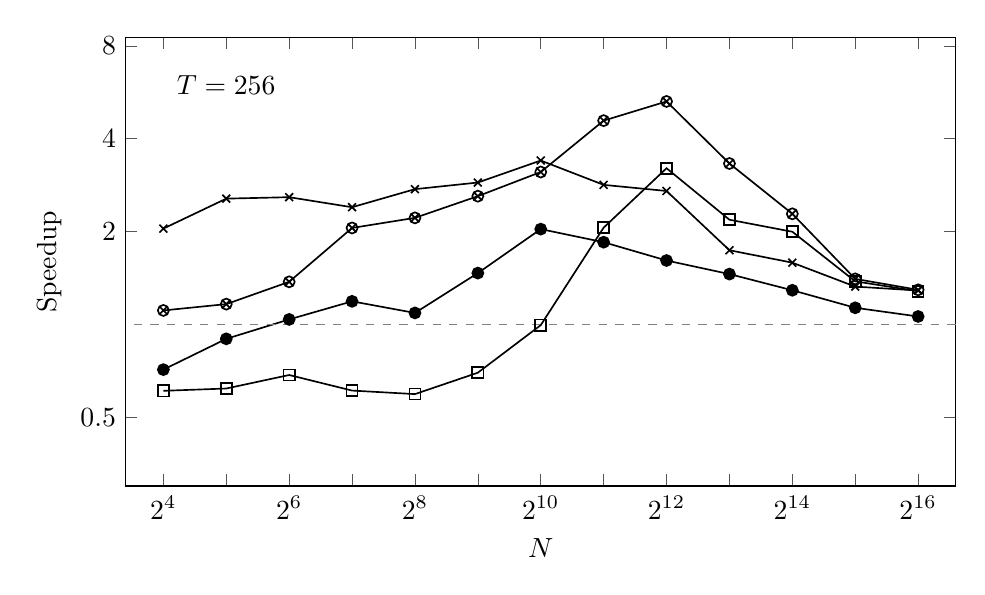
\begin{tikzpicture}

\begin{axis}[
axis line style={black},
xlabel={$N$},
xlabel near ticks,
xmin=-0.6, xmax=12.6,
xtick style={color=white!33.3333333333333!black},
xtick={0,1,2,3,4,5,6,7,8,9,10,11,12},
xticklabels={\(\displaystyle 2^4\),\(\),\(\displaystyle 2^6\),\(\),\(\displaystyle 2^8\),\(\),\(\displaystyle 2^{10}\),\(\),\(\displaystyle 2^{12}\),\(\),\(\displaystyle 2^{14}\),\(\),\(\displaystyle 2^{16}\)},
ylabel={Speedup},
ylabel near ticks,
ytick style={color=white!33.3333333333333!black},
%ytick={0,1,2,3,4,5,6},
%yticklabels={,\(\displaystyle {1.0}\),,\(\displaystyle {3.0}\),,\(\displaystyle {5.0}\),},
%ymin=0.361127455148372, ymax=5.51707532158344,
ymin=0.3, ymax=8.5,
ymode=log,
log basis y={2},
ytick={0.5,2,4,8},
log ticks with fixed point,
width=\textwidth,
height=0.6\textwidth,
title={$T=256$},
title style={below right,at={(0.05,0.9)}}
]
\addplot [semithick, mark=otimes]
table {%
0 1.11147540983607
1 1.16501650165017
2 1.37581699346405
3 2.05629139072848
4 2.21710526315789
5 2.60615384615385
6 3.12078651685393
7 4.57857142857143
8 5.2827140549273
9 3.32571109871723
10 2.28499799438428
11 1.40641665600068
12 1.29619187709406
};
% \addlegendentry{B1}
\addplot [semithick, mark=square]
table {%
0 0.610244988864143
1 0.620842572062084
2 0.686666666666667
3 0.611408199643494
4 0.595488721804511
5 0.698653198653199
6 0.995929443690638
7 2.06111111111111
8 3.21023359288098
9 2.18633540372671
10 1.99912018300194
11 1.38082448735985
12 1.28262231666122
};
% \addlegendentry{B2}
\addplot [semithick, mark=x]
table {%
0 2.04658385093168
1 2.55905511811024
2 2.58680555555556
3 2.4
4 2.74642857142857
5 2.88562091503268
6 3.40054495912806
7 2.83580080753701
8 2.70911949685535
9 1.74132043255549
10 1.58726097495287
11 1.32766260484254
12 1.2893861343636
};
% \addlegendentry{B3}
\addplot [semithick, mark=*]
table {%
0 0.714707329070339
1 0.899248120300752
2 1.03947368421053
3 1.18948412698413
4 1.09095002251238
5 1.46853146853147
6 2.03842794759825
7 1.84909727836163
8 1.61319515399212
9 1.45761636107193
10 1.29182463005992
11 1.13366620453858
12 1.06254475718846
};
% \addlegendentry{B4}
\addplot[gray, dashed] coordinates {(-1,1) (13,1)};
\end{axis}

\end{tikzpicture}
}}
\subfloat[]{\resizebox{0.45\textwidth}{!}{% This file was created by tikzplotlib v0.9.2.
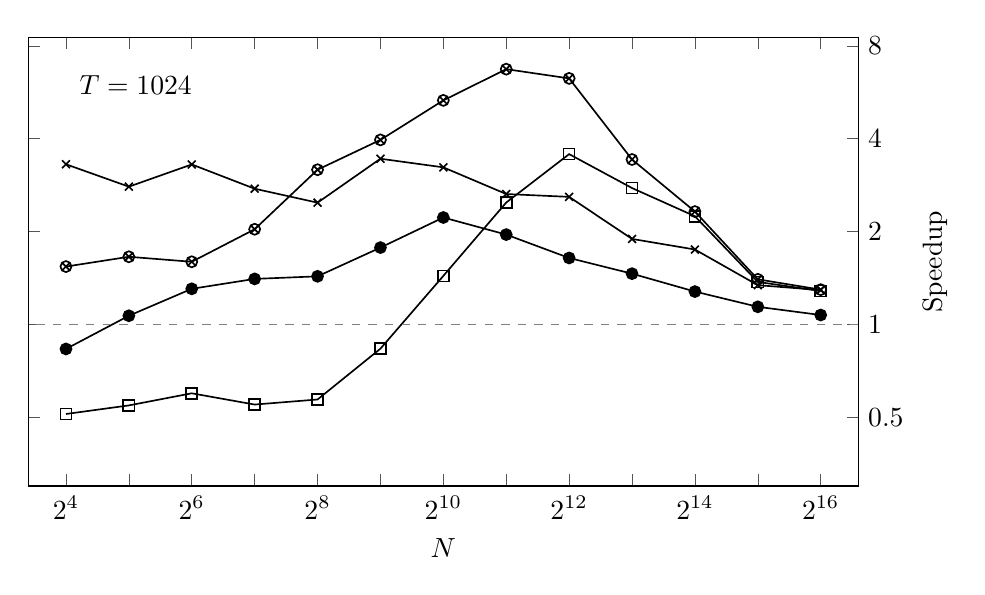
\begin{tikzpicture}

\begin{axis}[
axis line style={black},
xlabel={$N$},
xmin=-0.6, xmax=12.6,
xlabel near ticks,
xtick style={color=white!33.3333333333333!black},
xtick={0,1,2,3,4,5,6,7,8,9,10,11,12},
xticklabels={\(\displaystyle 2^4\),\(\),\(\displaystyle 2^6\),\(\),\(\displaystyle 2^8\),\(\),\(\displaystyle 2^{10}\),\(\),\(\displaystyle 2^{12}\),\(\),\(\displaystyle 2^{14}\),\(\),\(\displaystyle 2^{16}\)},
ylabel={Speedup},
ylabel near ticks,
%ymin=0.202966825333382, ymax=7.6,
ytick style={color=white!33.3333333333333!black},
%yticklabels={,\(\displaystyle {1.0}\),,\(\displaystyle {3.0}\),,\(\displaystyle {5.0}\),,\(\displaystyle {7.0}\),\(\displaystyle {8.0}\)},
ymode=log,
log basis y={2},
ymin=0.3, ymax=8.5,
ytick={0.5,1,2,4,8},
log ticks with fixed point,
yticklabel pos=right,
width=\textwidth,
height=0.6\textwidth,
title={$T=1024$},
title style={below right,at={(0.05,0.9)}}
]
\addplot [semithick, mark=otimes]
table {%
0 1.54172560113154
1 1.65860215053763
2 1.59782608695652
3 2.03624161073826
4 3.17523056653491
5 3.96593673965937
6 5.32525951557093
7 6.72148541114058
8 6.2743450321305
9 3.42638125542378
10 2.32380177063193
11 1.40163487155345
12 1.29789579295094
};
% \addlegendentry{B1}
\addplot [semithick, mark=square]
table {%
0 0.513372472276582
1 0.547333333333333
2 0.599075297225892
3 0.550828729281768
4 0.57201646090535
5 0.835728952772074
6 1.43811764705882
7 2.48555411815438
8 3.56691152986266
9 2.76931747025673
10 2.24389385867926
11 1.37479676536026
12 1.28436651244046
};
% \addlegendentry{B2}
\addplot [semithick, mark=x]
table {%
0 3.30685203574975
1 2.79770114942529
2 3.30263157894737
3 2.75550891920252
4 2.48282630029441
5 3.44634377967711
6 3.23179190751445
7 2.64840182648402
8 2.59288461538462
9 1.89490421158768
10 1.7509535977484
11 1.34198274819622
12 1.29377530790229
};
% \addlegendentry{B3}
\addplot [semithick, mark=*]
table {%
0 0.833864844343204
1 1.06823060410917
2 1.30601343101343
3 1.40609367894497
4 1.4334323922734
5 1.77639399943391
6 2.22291134622401
7 1.9573504027618
8 1.64384220061375
9 1.46215812497777
10 1.27950960037583
11 1.14186188461619
12 1.07420840134936
};
% \addlegendentry{B4}
\addplot[gray, dashed] coordinates {(-1,1) (13,1)};
\end{axis}

\end{tikzpicture}
}}
\caption[]{Speedup of concurrent execution with hidden helper tasks compared to vanilla LLVM with different benchmarks.}
\label{fig:speedup-nw-vanilla}
\end{figure}

\paragraph{Recent Progress}
In recent work we implemented loop transformation constructions introduced in OpenMP 5.1~\cite{kruse2021openmpbooth,kruse2021clangast}, asynchronous offloading for OpenMP~\cite{thiddenhelper}, efficient lowering of idiomatic OpenMP code to GPUs (under review),  OpenMP-aware compiler optimizations with informative and actionable remarks for users (under review), a portable OpenMP device (=gpu) runtime written in OpenMP 5.1 (including atomic support)~\cite{DBLP:conf/iwomp/TianCDC21}, a virtual GPU as debugging friendly
offloading target on the host~\cite{DBLP:conf/icppw/PatelTDC21}, improved diagnostics and execution information~\cite{DBLP:conf/icppw/DoerfertHC21,DBLP:conf/iwomp/HuberWGDH21}.

We implemented hidden helper task design in LLVM/OpenMP.
Most of our work \cite{DBLP:conf/iwomp/TianCDC21} (except device side dependence resolution) have been upstream and already part of LLVM since 12.0.
Recently Intel also adopted our design and implementation in Intel's latest OpenMP compiler \cite{TianUpdateOnIntelCompiler2021}.

The loop transformation constructs implemented in Clang include the \emph{unroll} and \emph{tile} directives.
We demonstrate how these make speedup in the vicinity of 3x (tiling) and 20\% become
low-hanging fruits by just adding a directive~\cite{kruse2021openmpbooth}.
There are actually two implementations, one AST-based and a second using the OpenMPIRBuilder that can also be used other compilers such as Flang~\cite{kruse2021clangast}.

Testing of OpenMP offloading for NVIDIA and AMD GPUs has been added to LLVM's Continuous Integration infrastructure.
This will allow identifying changes that break OpenMP early during development, including those by non-OpenMP developers making maintenance easier.

GPU kernel times have been improved significantly since LLVM 12. \autoref{fig:kernel_times} illustrates the impact of
different optimizations we integrated into LLVM and which are run by default for OpenMP codes. As shown, speedups
of up to 13.35x (RSBench, upper right) were reached while we get closer to CUDA
performance across the board. More recent improvements caused benchmarks like
XSBench (upper left) to also achieve CUDA performance when compiled with OpenMP
offload via our development branch of LLVM/Clang.

\begin{figure}[hbt!]
\centering
\includegraphics[width=0.95\linewidth]{projects/2.3.2-Tools/2.3.2.11-SOLLVE/LLVM-Implementation-Figures/LLVM-opt-kernel-times.jpg}
\caption[]{Kernel times for different ECP proxy apps when compiled with OpenMP offloading and CUDA. For the former differently optimized versions are shown and the results of a close to LLVM upstream branch is marked explicitly. All times are normalized against LLVM 12 OpenMP offloading performance.}
\label{fig:kernel_times}
\end{figure}

LLVM/Clang 13.0.0 has been officially released on October 4 which includes most of the aforementioned improvements.


\paragraph{Next Steps}
We will keep working on supporting more new OpenMP 5.1 features in LLVM.
%OpenMP 5.1 introduces a number of new features, one of which is new set of useful atomic operations, \lstinline{compare} clause and a combined one \lstinline{compare capture}.
%Now most of atomic operations in scientific applications can be written in OpenMP directly instead of using target dependent intrinsics or function calls.
%We will support the two clauses in LLVM/Clang.
%
To avoid redundant development of two OpenMP implementations, we will mature the development of the OpenMPIRBuilder and make it the default OpenMP code generation for Clang as it is already for Flang.

Improvements to the OpenMP offloading ecosystem are planned, e.g., to extend the remote offloading capabilities we introduced and to further improve development and debugging of OpenMP GPU applications.

More OpenMP-aware optimizations are expected to materialize as we get the last OpenMP benchmarks on par with CUDA performance. We also plan to invest time in generic GPU optimizations soon.
